\section{Theorie}
\label{sec:Theorie}

\subsection{Suszeptibilität paramagnetischer Substanzen}

Für das magnetische Feld im Vakuum lässt sich die magnetische Flussdichte $\vec{B}$ durch die magnetische Feldstärke $\vec{H}$ ausdrücken:

\begin{equation}
    \vec{B} = \mu_0 \vec{H}
\end{equation}

Hierbei ist $\mu_0$ die Induktionskonstante.\\
Passiert das magnetische Feld Materie, so kommt zu $\vec{B}$ noch die Magnetisierung $\vec{M}$ dazu:

\begin{equation}
    \vec{B} = \mu_0 \vec{H}\ +\ \vec{M}
\end{equation}

Die Magnetisierung kann über die Suszeptibilität $\chi$ berechnet werden:

\begin{equation}
    \vec{M} = \mu_0 \chi \vec{H}
\end{equation}

Die Suszeptibilität ist hierbei keine Konstante, sondern stark von der Temperatur abhängig.\\
Die meiste Materie ist diamagnetisch, nur solche Materie mit nicht verschwindendem Drehimpuls in dessen Atomen ist paramagnetisch.
Da die Bewegung der Atome hauptsächlich thermisch ist, verändern sich die Drehmomente mit der Temperatur.\\
Der atomare Drehimpuls setzt sich aus drei Komponenten zusammen:
\begin{itemize}
    \item Bahndrehimpuls der Elektronenhülle
    \item Spin der Elektronen
    \item Kerndrehimpuls
\end{itemize}
Wenn das Magnetfeld, welches die Materie durchdringt nicht allzu stark ist, kann der Kerndrehimpuls vernachlässigt werden.
Für den Gesamtdrehimpuls $\vec{J}$ muss nun die Vektorsumme des Gesamtbahndrehimpulses $\vec{L}$ und der Spins $\vec{S}$ addiert werden.

\begin{equation}
    \vec{J} = \vec{L}\ +\ \vec{S}
\end{equation}

Aus den Impulsen lassen sich die magnetischen Momente berechnen:

\begin{equation}
    \vec{\mu}_L = -\frac{\mu_B}{\hbar}\vec{L}
\end{equation}

und

\begin{equation}
    \vec{\mu}_S = -g_S\frac{\mu_B}{\hbar}\vec{S}
\end{equation}

Dabei ist $\mu_B$ das Bohrsche Magneton mit 

\begin{equation}
    \mu_B = \frac{1}{2}\frac{e_0}{m_0}\hbar
\end{equation}

und $g_S$ das gyromagnetische Verhältnis.\\
Um den Betrag des magnetischen Moments von $\vec{\mu}_J$ zu erhalten, müssen zunächst die Beträge von $\vec{\mu}_S$ und $\vec{\mu}_L$ ermittelt werden und gemäß der geometrischen Anordnung der Drehmomente und magnetischen Momente verrechnet werden.\\
Die Formeln für $|\vec{\mu}|$ lauten:

\begin{align*}
    \mid\vec{\mu}_L\mid = \mu_B \sqrt{L(L\ +\ 1)}\\
    \text{und     }\\
    \mid\vec{\mu}_S\mid = g_S \mu_B \sqrt{S(S\ +\ 1)}
\end{align*}

Anhand \autoref{fig:theo} lässt sich die Berechnung von $\mid \vec{\mu}_J \mid$ nachvollziehen.

\begin{figure}[htbp]
    \centering
    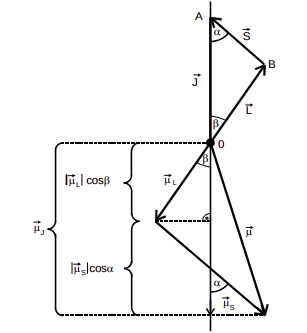
\includegraphics[scale=0.8]{Data/Theobild.png}
    \caption{Vektordiagramm der Drehimpulsvektoren und den daraus hervorgehenden magnetischen Momenten.}
    \label{fig:theo}
\end{figure}

Demnach ergibt sich für $\mid\vec{\mu}_J\mid$:
\begin{equation}
    \mid\vec{\mu}_J\mid = \mid\vec{\mu}_S\mid \cos\alpha \ +\ \mid\vec{\mu}_L\mid \cos\beta
\end{equation}

Werden die Werte für $|\vec{\mu}_{S,L}|$ zusammen mit den geometrischen Formeln für $\cos\alpha$ und $\cos\beta$ einsetzt und beachtet, dass $g_S \approx 2$, dann ergibt sich eine neue Formel für $|\vec{\mu}_J|$:

\begin{equation}
    |\vec{\mu}_J| \approx \mu_B \underbrace{\sqrt{J(J+1)}\frac{3J(J+1)\ +\ [S(S+1)\ -\ L(L+1)]}{2J(J+1)}}_{:=g_J}
\end{equation}
Da der Versuch mit makroskopischen Messungen zu tun hat, wird eine Berechnung der makroskopischen Magnetisierung benötigt.

\begin{equation}
    M = \mu_0 N \bar{\mu}
\end{equation}

\begin{equation}
    \bar{\mu} = -\mu_Bg_J\frac{\sum_{m=-J}^J m\cdot \exp(\frac{-\mu_Bg_JmB}{kT})}{\sum_{m=-J}^J \exp(\frac{-\mu_Bg_JmB}{kT})}
    \label{eq:mitmag}
\end{equation}

Hierbei ist $\bar{\mu}$ das mittlere magnetische Moment und wird nach \autoref{eq:mitmag} berechnet.\\
Nach Anwendung einer Hochtemperaturnäherung lässt sich schließlich eine Formel für $\chi$ bestimmen:

\begin{equation}
    \chi = \frac{\mu_0 \mu_B^2 g_J^2 N J(J+1)}{3kT}
    \label{eq:chitheo}
\end{equation}

Aus dieser Formel geht hervor, dass $\chi \sim 1/T$. Dies ist das Curiesche Gesetz des Paramagnetismus.


\newpage
\subsection{Suszeptibilität von Seltenen-Erd-Verbindungen}
Seltene-Erd-Verbindungen zeigen einen starken Paramagnetismus, was bedeuten muss, dass die Atome große Drehimpulse besitzen.
Diese Drehimpulse können nur die inneren Elektronen Erzeugen, genauer die sogenannten 4f-Elektronen.
Das 4f ist dabei eine Zuordnung zu einer Schale in der die Elektronen energetisch liegen.\\
Der von ihnen erzeugte Drehimpuls $\vec{J}$ kann mit den Hundschen Regeln bestimmt werden.
Diese sagen aus:
\begin{itemize}
    \item Die Spins $\vec{s}_i$ kombinieren zum maximalen Gesamtspin $\vec{S} = \sum \vec{s}_i$, der nach dem Pauli-Prinzip möglich ist.
    \item Die Bahndrehimpulse $\vec{l}_i$ setzen sich so zusammen, dass der maximale Drehimpuls $\vec{L} = \sum \vec{l}_i$, der mit dem Pauli-Prinzip und der Regel 1 verträglich ist, entsteht.
    \item Der Gesamtdrehimpuls ist $\vec{J} = \vec{L}-\vec{S}$, wenn die Schale weniger als halb und $\vec{J} = \vec{L}+\vec{S}$, wenn die Schale mehr als halb gefüllt ist.
\end{itemize}
Mit diesen Regeln lässt sich $g_J$ aus \autoref{eq:chitheo} bestimmen.

\subsection{Berechnung mittels einer Brückenschaltung}
Die Suszeptibilität kann auch anders berechnet werden, indem eine Brückenschaltung mit integrierter Spule aufgebaut wird und die paramagnetischen Materialien das Magnetfeld direkt beeinflussen und somit auch die Brückenspannung und erforderlichen Widerstand.
Ist die Messfrequenz dabei deutlich höher als der fest verbaute Widerstand in der Brückenschaltung, so lässt sich bei bekannter Brücken- und Speisespannung $\chi$ ausrechnen:
\begin{equation}
    \chi_U = 4\frac{F}{Q}\frac{U_{Br}}{U_{Sp}}
    \label{eq:chiu}
\end{equation}
Hierbei ist F der Spulenquerschnitt und Q der Probenquerschnitt.\\
Eine weitere Messmethode funktioniert über den verstellbaren Widerstand, üblicherweise $R_3$, und dessen Unterschied im Wert, mit und ohne Probe, $\Delta R$.
\begin{equation}
    \chi_R = 2\frac{\Delta R}{R_3}\frac{F}{Q}
    \label{eq:chir}
\end{equation} 
